\section{Moments}

\boxdefinition{Moment}{
    Let $X$ be a continuous random variable with PDF $f(x)$. The $k^{th}$ moment of $X$ (if it exists) is
    \begin{equation*}
        \E[X^k] = \int_{-\infty}^{\infty} x^k \cdot f(x) \ dx
    \end{equation*}
}
Th expected value of a random variable is its first moment.
\boxdefinition{Central moment}{
    Let $X$ be a continuous random variable with PDF $f(x)$. The $k^{th}$ central moment of $X$ (if it exists) is
    \begin{equation*}
        \mu_k = \E[(X - \mu)^k] = \int_{-\infty}^{\infty} (x - \mu)^k f(x) \ dx
    \end{equation*}
}
The variance of a random variable is its second central moment. \\
Another related concept is the $k^{th}$ standardized moment, which is the $k^{th}$ central moment divided by the standard deviation raised to the $k^{th}$ power:
\begin{equation*}
    \tilde{\mu}_k = \frac{\mu_k}{\sigma^k} = \E\left[\left(\frac{X-\mu}{\sigma}\right)^k\right]
\end{equation*}
\begin{itemize}
    \item $\tilde{\mu}_1 = 0$ (since $\E[X - \mu] = 0$ for any random variable);
    \item $\tilde{\mu}_2 = 1$ (since $\E[(X - \mu)^2] = \sigma^2$);
    \item $\tilde{\mu}_3$ is called \textbf{skewness} and measures the magnitude and direction of the asymmetry of the distribution. If it is 0, the distribution is symmetric, and mean, median, and mode coincide. If it is positive, the distribution is \textbf{right-skewed} (the mean is greater than mode and median), while if it is negative, the distribution is \textbf{left-skewed} (the mean is less than mode and median).
    \begin{figure}[ht]
        \centering
        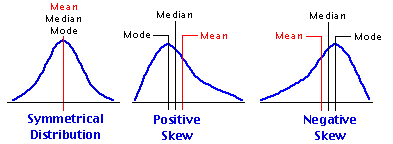
\includegraphics[width=0.7\textwidth]{img/skew.png}
        \caption{Skewness of distributions.}
    \end{figure}
    \item $\tilde{\mu}_4$ is called \textbf{kurtosis} and measures the dispersion of the random variable around the values $\mu+\sigma$ and $\mu - \sigma$. Specifically, the kurtosis of a distribution is compared to that of a Normal distribution, which is always 3. Then, if the kurtosis is equal to 3, the distribuion is \textbf{mesokurtic} (similar to a Normal); if it is greater than 3, it is \textbf{leptokurtic} (the tails are fatter, while the middle is thinner); if it is less than 3, it is \textbf{platykurtic} (the tails are thinner, but the middle is larger).
\end{itemize}